\documentclass{beamer}

\usepackage[utf8]{inputenc}
\usepackage{tikz}
\usepackage{natbib}
\usepackage{graphicx}
\usepackage{amsmath}
\usepackage{amssymb}
\usepackage{amsfonts}
%\usepackage{algorithm}
%\usepackage{algorithmic}
\usepackage{setspace}
\usepackage{subfig}
\usepackage{adjustbox}
\usepackage{tikz}
\usepackage{xcolor}

%math fonts a
\usefonttheme[onlymath]{serif}

\usetikzlibrary{arrows,automata,positioning}
\usetikzlibrary{shapes.multipart}
\usetikzlibrary{decorations.markings}
\usetikzlibrary{decorations.pathreplacing}

\makeatletter
\def\th@mystyle{
    %\normalfont % body font
    \setbeamercolor{block title example}{bg=myred,fg=white}
    \setbeamercolor{block body example}{bg=lightgray!20,fg=black}
    \def\inserttheoremblockenv{exampleblock}
  }
\makeatother
\theoremstyle{mystyle}
\newtheorem*{remark}{Remark}

\usetheme{metropolis} 
\usecolortheme{beaver}
\fontfamily{verdana}

\definecolor{myred}{HTML}{cc0000}
\definecolor{mygreen}{HTML}{009B55}

% THEME
\setbeamertemplate{itemize item}{\color{myred}\bf{-}}
\setbeamertemplate{itemize subitem}{\color{myred}$\blacktriangleright$}
\setbeamercolor{item in toc}{fg=myred}
\setbeamercolor{title}{fg=black}

\setbeamercolor{frametitle}{fg=myred}
\setbeamerfont{footnote}{size=\tiny}

\metroset{sectionpage=none, progressbar=frametitle, numbering=fraction}


\usetikzlibrary{arrows,automata,positioning}
\usetikzlibrary{shapes.multipart}
\usetikzlibrary{decorations.markings}
\usetikzlibrary{decorations.pathreplacing}


% macros:
\newcommand{\tS}{\text{t}}   % for terminal states
\newcommand{\cA}{\mathcal{A}}
\newcommand{\cB}{\mathcal{B}}
\newcommand{\cC}{\mathcal{C}}
\newcommand{\cD}{\mathcal{D}}
\newcommand{\cE}{\mathcal{E}}
\newcommand{\cJ}{\mathcal{J}}
\newcommand{\cL}{\mathcal{L}}
\newcommand{\cM}{\mathcal{M}}
\newcommand{\cP}{\mathcal{P}}
\newcommand{\cR}{\mathcal{R}}
\newcommand{\cS}{\mathcal{S}}
\newcommand{\cT}{\mathcal{T}}
\newcommand{\cU}{\mathcal{U}}
\newcommand{\cV}{\mathcal{V}}
\newcommand{\cX}{\mathcal{X}}

\newcommand{\EE}[1]{\mathbb{E}\left[#1\right]}
\newcommand{\EEc}[2]{\mathbb{E}\left[#1\;\middle\lvert\;#2\right]}
\newcommand{\pa}[1]{\left(#1\right)}

\newcommand{\diag}{\text{diag}}
\newcommand{\real}{\mathbb{R}}

\titlegraphic{%
  \hspace{10em}
\includegraphics[width=3cm,height=1.6cm,keepaspectratio]{Figures/upf_logo.png}\hfill
}

\title[Globally Optimal HRL for LMDPs]{Globally Optimal Hierarchical Reinforcement Learning for Linearly-Solvable Markov Decision Processes}
\author[G. Infante, A. Jonsson, V. Gómez ]{Guillermo Infante, Anders Jonsson, Vicenç Gómez}
\date[]{\textit{AAAI 2022}}


\begin{document}

\begin{frame}
    \maketitle
\end{frame}

\begin{frame}{Overview}
    \tableofcontents
\end{frame}

\section{Hierarchical RL and recursive \textit{optimality}}

\begin{frame}{Hierarchical RL and recursive \textit{optimality}}

    \begin{figure}
        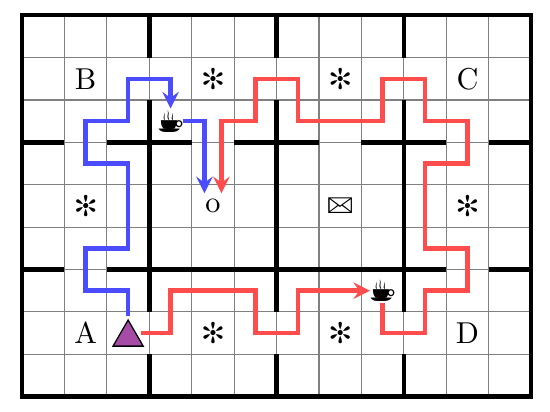
\includegraphics[width=0.4\textwidth]{Figures/coffee.png}
        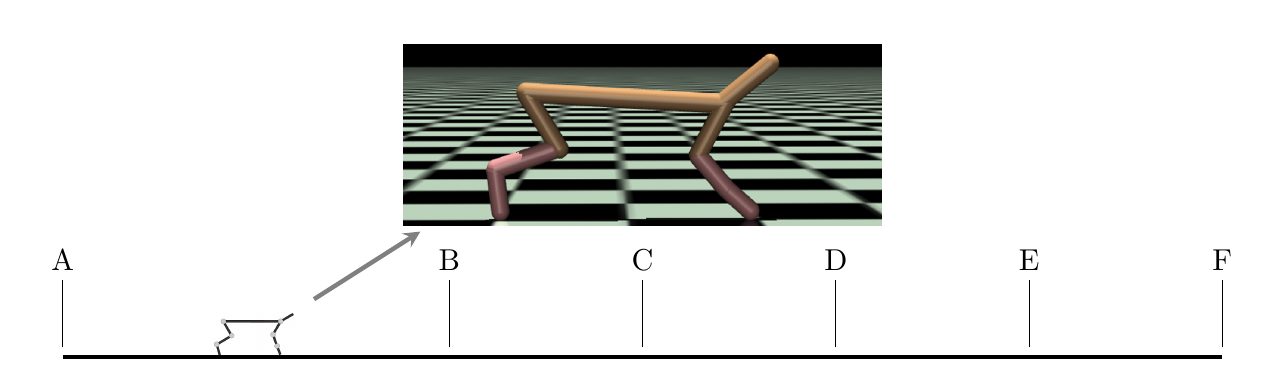
\includegraphics[width=0.8\textwidth]{Figures/cheetah.png}
        \caption*{\citep{Icarte2022}}
    \end{figure}
\end{frame}

\section{Compositionality}


\begin{frame}{\textit{Compositionality} in RL}

    \begin{itemize}
        \item In general, in standard RL settings
              \[Q_A(s, a) \circ Q_B(s, a) \neq Q_{A\circ B}(s, a).
              \]
        \item \textit{Possible} under some assumptions (\textit{entropy-regularization}).
    \end{itemize}
    \begin{figure}
        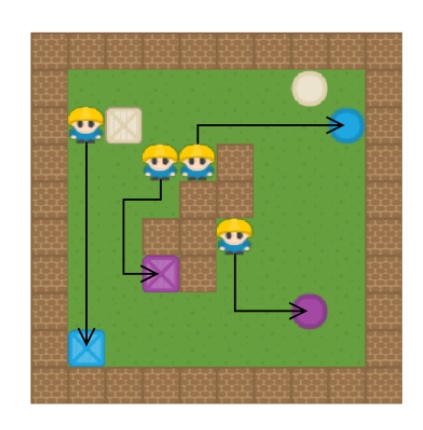
\includegraphics[width=0.5\textwidth, height=0.4\textwidth]{Figures/composable.png}
        \caption*{\citep{Niekerk2019}}
    \end{figure}

\end{frame}

\begin{frame}{Question?}
    Is there a way to combine {\bf \color{blue} hierarchical representations and \textit{compositionality}} to make more {\bf \color{mygreen} sample efficient algorithms} while preserving {\bf optimal solutions}?
\end{frame}

\section{Linearly-solvable MDPs (LMDPs)}
\begin{frame}{Definition of a LMDP}
    We define an LMDP~\citep{Kappen2012,Todorov2006} as a tuple $\cL=\langle {\color{blue} \cS,\cT}, {\color{orange} \cP}, {\color{myred}\cR},{\color{mygreen}\cJ}\rangle$:
    \begin{itemize}
        \item Let ${\color{blue}\cS^+=\cS\cup\cT}$.
        \item ${\color{orange}\cP:\cS\rightarrow\Delta(\cS^+)}$, ${\color{myred}\cR:\cS\rightarrow\real}$ and ${\color{mygreen}\cJ:\cT\rightarrow\real}$.
        \item Learning agent follows a policy $\pi:\cS\rightarrow\Delta(\cS^+)$.
    \end{itemize}

    At time-step $t$, the agent observes $s_t$ and receives a reward \[ \cR(s_t,\pi) = \cR(s_t) - \lambda\cdot\mathrm{KL}(\pi(\cdot|s_t)\Vert\, \cP(\cdot|s_t))\] and travels to $s_{t+1} \sim \pi(\cdot\lvert s_t)$.

\end{frame}

\begin{frame}{The learning objective}

    \begin{itemize}

        \item The aim of the agent is to maximize \[ v^\pi(s) = \EEc{\sum_{t=1}^{T-1} \cR(S_t,\pi) + \cJ(S_T)}{S_1 = s}.\]
        \item We obtain the following Bellman optimality equation
              \begin{equation*}
                  \frac 1 \lambda v(s) = \frac 1 \lambda \cR(s) + \max_\pi \mathbb{E}_{s'\sim\pi(\cdot|s)} \left[ \frac 1 \lambda v(s') - \log \frac {\pi(s'|s)} {\cP(s'|s)} \right] \;\; (\forall s).
              \end{equation*}

    \end{itemize}
\end{frame}

\begin{frame}{Solving an LMDP}

    {\bf Dynamic programming}

    \begin{itemize}
        \item Taking $z(s)=e^{v(s)/\lambda}$ for each $s\in\cS^+$ leads to
    \end{itemize}
    \[ z(s) = e^{\cR(s)/\lambda} \sum_{s'}\cP(s'|s)z(s') \   \longrightarrow \ \mathbf{z} = R P \mathbf{z}\]
    {\bf Online update rule}
    \[ \hat{z}(s_t) \leftarrow \hat{z}(s_t) + {\pmb{\alpha_t}} \Big({\color{blue} \frac {\cP(s_{t+1}|s_t)} {\hat{\pi}(s_{t+1}|s_t)}} e^{r_t/\lambda}\hat{z}(s_{t+1}) - \hat{z}(s_t) \Big), \]
    to learn from samples $(s_t, r_t, s_{t+1})$.

    %\item Given a $z$, policies are derived using \[ \pi(s'|s) = \frac {\cP(s'|s)z(s')} {\sum_{s''} \cP(s''|s)z(s'')}.\]

\end{frame}

\begin{frame}{Compositionality in LMDPs}
    \begin{itemize}
        \item Let $\{\cL_1,\ldots,\cL_n\}$ be a collection of LMDPs.

        \item Each LMDP $\cL_i$ {\color{blue} only differs in $\cJ_i(\tS)$}.

        \item For a new LMDP $\cL$ for which the next holds,
              \begin{equation*}
                  e^{\cJ(\tS)/\lambda} = z(\tS) = \sum_{k=1}^n {\color{blue} w_k} e^{\cJ_k(\tS)/\lambda} \ \text{for} \ \tS \in \cT_i.
              \end{equation*}

        \item Due to linearity, the following is also satisfied

              \begin{equation*}
                  z(s) =  \sum_{k=1}^n {\color{blue} w_k} z_k(s) \ \forall s \in \cS.
              \end{equation*}

    \end{itemize}

\end{frame}

\section{Hierarchical compositionality with LMDPs}
\begin{frame}{Hierarchical LMDPs (i)}

    \begin{itemize}
        \item For an LMDP $\cL$, its {\color{blue} $\cS$ is partitioned} into $L$ subsets $\{\cS_i\}_{i=1}^L$.
        \item Each $\cS_i$ induces a subtask $\cL_i=\langle\cS_i,\cT_i,\cP_i,\cR_i,\cJ_i\rangle$:
              \begin{itemize}
                  \item $\cT_i$ includes states in $\cS^+\setminus\cS_i$ that are one step away from any $s \in \cS_i$.
                  \item For $\tau\in\cT_i$,
                        \[
                            \cJ_i(\tau)=\begin{cases}
                                \cJ(\tau) \ \text{if} \ \tau\in\cT, \\
                                \hat{v}(\tau) \ \text{otherwise.}
                            \end{cases}
                        \]
              \end{itemize}
    \end{itemize}

\end{frame}

\begin{frame}{Hierarchical LMDPs (ii)}

    \begin{definition}
        Subtask equivalence (for some $\cL_i$ and $\cL_j$) imples a bijective relationship $f:\cS_i\rightarrow\cS_j$.
    \end{definition}

    \begin{itemize}

        \item Set of  {\color{blue}{\em exit states}} $\cE=\cup_{i=1}^L\cT_i$
        \item $\cE_i=\cE\cap\cS_i$ denotes the set of {\color{blue}{\em exit states inside}} subtask $\cL_i$.
        \item Set of {\color{blue} equivalence classes} $\cC=\{\cC_1,\ldots,\cC_C\}$, $C\leq L$.
        \item {\color{blue} A single subtask} $\cL_j=\langle\cS_j,\cT_j,\cP_j,\cR_j,\cJ_j\rangle$ {\color{blue} per equivalence class} $\cC_j\in\cC$.

    \end{itemize}


\end{frame}

\begin{frame}{Hierarchical LMDPs (iii) - Illustration}

    \begin{figure}
        \begin{center}
            \begin{tikzpicture}
                \draw[step=0.4,thin,shift={(0.2,0.2)}] (0.8,0.8) grid (4.8,4.8);
                \draw[ultra thick] (1,1) rectangle (5,5);
                \draw[ultra thick] (3,1) -- (3,1.8);
                \draw[ultra thick] (3,2.2) -- (3,3.8);
                \draw[ultra thick] (3,4.2) -- (3,5);
                \draw[ultra thick] (1,3) -- (1.8,3);
                \draw[ultra thick] (2.2,3) -- (3.8,3);
                \draw[ultra thick] (4.2,3) -- (5,3);

                \draw[fill] (0.6,1.8) rectangle (1,2.2);
                \draw[fill] (0.6,3.8) rectangle (1,4.2);
                \draw[fill] (1.8,5) rectangle (2.2,5.4);
                \draw[fill] (1.8,0.6) rectangle (2.2,1);
                \draw[fill] (3.8,0.6) rectangle (4.2,1);
                \draw[fill] (5,1.8) rectangle (5.4,2.2);
                \draw[fill] (5,3.8) rectangle (5.4,4.2);
                \draw[fill] (3.8,5) rectangle (4.2,5.4);

                \draw[fill] (2.2,2.2) rectangle (2.6,2.6);
                \draw[fill] (4.2,2.2) rectangle (4.6,2.6);
                \draw[fill] (2.2,4.2) rectangle (2.6,4.6);


                \draw[ultra thick] (4.2,4.2) rectangle (4.6,4.6);
                \draw[ultra thick] (3.8,2.6) rectangle (4.2,3.4);
                \draw[ultra thick] (1.8,2.6) rectangle (2.2,3.4);
                \draw[ultra thick] (2.6,3.8) rectangle (3.4,4.2);
                \draw[ultra thick] (2.6,1.8) rectangle (3.4,2.2);

                \node at (4.4,4.4) {\small $G$};
                \node at (2,3.2) {\small $2^T$};
                \node at (2,2.8) {\small $1^B$};
                \node at (4,3.2) {\small $4^T$};
                \node at (4,2.8) {\small $3^B$};
                \node at (2.8,4) {\small $3^L$};
                \node at (2.8,2) {\small $4^L$};
                \node at (3.2,4) {\small $1^R$};
                \node at (3.2,2) {\small $2^R$};

                \draw[step=0.4,thin,shift={(0.2,0)}] (8.799,1.999) grid (10.8,4);
                \draw[ultra thick] (9,3.2) -- (8.6,3.2) -- (8.6,2.8) -- (9,2.8) -- (9,2) -- (9.8,2);
                \draw[ultra thick] (9,3.2) -- (9,4) -- (9.8,4) -- (9.8,4.4) -- (10.2,4.4) -- (10.2,4);
                \draw[ultra thick] (10.2,4) -- (11,4) -- (11,3.2) -- (11.4,3.2) -- (11.4,2.8) -- (11,2.8);
                \draw[ultra thick] (9.8,2) -- (9.8,1.6) -- (10.2,1.6) -- (10.2,2) -- (11,2) -- (11,2.8);
                \draw[ultra thick] (10.2,3.2) rectangle (10.6,3.6);

                \node at (10.4,3.4) {\small $G$};
                \node at (8.8,3)    {\small $L$};
                \node at (11.2,3)   {\small $R$};
                \node at (10,1.8)   {\small $B$};
                \node at (10,4.2)   {\small $T$};

                \node at (3,0.7) {a)};
                \node at (10,0.7) {b)};
            \end{tikzpicture}
        \end{center}
        \caption{a) A 4-room LMDP, with all exit states highlighted; b) a single subtask with 5 terminal states $G,L,R,T,B$ that is equivalent to all 4 room subtasks.}
    \end{figure}

\end{frame}

\begin{frame}{Hierarchical LMDPs (iv) - Subtask compositionality (i)}

    \begin{itemize}
        \item Consider subtask $\cL_j$ and its terminal set~$\cT_j=\{\tau_1,\ldots,\tau_n\}$.
        \item We define {\color{blue} $n$ base LMDPs $\cL_j^1,\ldots,\cL_j^n$}, which only differ in $\cJ_j^k$.
        \item Concretely,
              \[
                  z_j^k(\tau)=\begin{cases}
                      1 \ \text{if} \ \tau=\tau_k \rightarrow \cJ_j^k(\tau)=0, \\
                      0 \ \text{otherwise} \ \rightarrow \cJ_j^k(\tau)=-\infty
                      %$z_j^k(\tau)=1$ if $\tau=\tau_k$, and $z_j^k(\tau)=0$ otherwise. This corresponds to an actual reward of $$ for $\tau=\tau_k$, and $$ otherwise.
                  \end{cases}
              \]
        \item Solutions are {\color{blue} optimal $z_j^1,\ldots,z_j^n$.}
        \item Having $\hat z(s)$ for each $t \in \cT_j$, {\color{blue}compositionality rule}
              \begin{equation*}
                  \hat{z}(s)=\hat{z}(\tau_1){\color{blue} z_j^1(s)}+\cdots+\hat{z}(\tau_n){\color{blue} z_j^n(s)} \;\; \forall s\in\cS_i,\forall\cL_i\in\cC_j.
              \end{equation*}
    \end{itemize}


\end{frame}


\begin{frame}{Hierarchical LMDPs (v) - Subtask compositionality (ii)}


    \begin{itemize}


        \item For all subtasks, terminal states $\tau_1 \dots \tau_n$ are by definition in $\cE$.
        \item Enough to represent $\hat z(s) \ \forall s \in \cS$:
              \begin{itemize}
                  \item $\hat{z}_\cE:\cE\rightarrow\mathbb{R}$,
                  \item for the base LMDPs {\color{blue} $z_j^1,\ldots,z_j^n$}.
              \end{itemize}
              %\item No need to store an explicit estimate $\hat z(s)$.
        \item Solutions for base LMDPs {\color{blue} can be reused}.

    \end{itemize}

\end{frame}


%\begin{frame}{Hierarchical LMDPs (vi) - Subtask compositionality (iii)}

%\begin{remark}[]
%    
%    If $\hat z(s)$ is optimal for $s \in \cE$, then $\hat z(s)$ for $s \in \cS_i$ will also be optimal. With compositionality, \[\hat z(s) = \hat z(3^L) * z_L(s) + \hat z(3^B) * z_B(s) + \hat z(G) * z_G(s)\]
%    
%    For any $s$ in $\cS_i$. Thus, if $\hat z = z^*$ for $s \in \cE$, then it will be optimal for the interior states as well.
%    
%    
%\end{remark}

%\begin{figure}
%\begin{center}
%
%\scalebox{0.6}{
%\begin{tikzpicture}
%\draw[step=0.4,thick,shift={(0.2,0.2)}] (0.8,0.8) grid (4.8, 4.8);
%\draw[step=0.4,thick,shift={(0.2,0.2)}, color=red] (2.8, 2.8) grid (4.8, 4.8);
%
%
%\draw[ultra thick] (1,1) rectangle (5,5);
%\draw[ultra thick] (3,1) -- (3,1.8);
%\draw[ultra thick] (3,2.2) -- (3,3.8);
%\draw[ultra thick, color=red] (3,3) -- (3,5);
%\draw[ultra thick] (1,3) -- (1.8,3);
%\draw[ultra thick] (2.2,3) -- (3.8,3);
%\draw[ultra thick, color=red] (3,3) -- (5,3);
%
%\draw[fill] (0.6,1.8) rectangle (1,2.2);
%\draw[fill] (0.6,3.8) rectangle (1,4.2);
%\draw[fill] (1.8,5) rectangle (2.2,5.4);
%\draw[fill] (1.8,0.6) rectangle (2.2,1);
%\draw[fill] (3.8,0.6) rectangle (4.2,1);
%\draw[fill] (5,1.8) rectangle (5.4,2.2);
%\draw[fill] (5,3.8) rectangle (5.4,4.2);
%\draw[fill] (3.8,5) rectangle (4.2,5.4);
%
%\draw[fill] (2.2,2.2) rectangle (2.6,2.6);
%\draw[fill] (4.2,2.2) rectangle (4.6,2.6);
%\draw[fill] (2.2,4.2) rectangle (2.6,4.6);
%
%\draw[ultra thick, color=red] (4.2,4.2) rectangle (4.6,4.6);
%\draw[ultra thick, color=red] (3.8,2.6) rectangle (4.2,3.4);
%\draw[ultra thick] (1.8,2.6) rectangle (2.2,3.4);
%\draw[ultra thick, color=red] (2.6,3.8) rectangle (3.4,4.2);
%\draw[ultra thick] (2.6,1.8) rectangle (3.4,2.2);
%
%\node at (4.4,4.4) {\small $G$};
%\node at (2,3.2) {\small $2^T$};
%\node at (2,2.8) {\small $1^B$};
%\node at (4,3.2) {\small $4^T$};
%\node at (4,2.8) {\small $3^B$};
%\node at (2.8,4) {\small $3^L$};
%\node at (2.8,2) {\small $4^L$};
%\node at (3.2,4) {\small $1^R$};
%\node at (3.2,2) {\small $2^R$};
%
%\draw[step=0.4,thin,shift={(0.2,0)}] (8.799,1.999) grid (10.8,4);
%\draw[ultra thick] (9,3.2) -- (8.6,3.2) -- (8.6,2.8) -- (9,2.8) -- (9,2) -- (9.8,2);
%\draw[ultra thick] (9,3.2) -- (9,4) -- (9.8,4) -- (9.8,4.4) -- (10.2,4.4) -- (10.2,4);
%\draw[ultra thick] (10.2,4) -- (11,4) -- (11,3.2) -- (11.4,3.2) -- (11.4,2.8) -- (11,2.8);
%\draw[ultra thick] (9.8,2) -- (9.8,1.6) -- (10.2,1.6) -- (10.2,2) -- (11,2) -- (11,2.8);
%\draw[ultra thick] (10.2,3.2) rectangle (10.6,3.6);
%
%\node at (10.4,3.4) {\small $G$};
%\node at (8.8,3)    {\small $L$};
%\node at (11.2,3)   {\small $R$};
%\node at (10,1.8)   {\small $B$};
%\node at (10,4.2)   {\small $T$};
%
%\end{tikzpicture}
%}
%\end{center}
%\end{figure}
%    
%\end{frame}
%

\begin{frame}{Eigenvector algorithm (i)}
    \begin{itemize}
        \item We can restrict
              \begin{equation*}
                  \hat{z}(s)=\hat{z}(\tau_1) {\color{blue} z_j^1(s)}+\cdots+\hat{z}(\tau_n){\color{blue}z_j^n(s)} \;\; \forall s\in\cS_i,\forall\cL_i\in\cC_j.
              \end{equation*}
              to states $s \in \cE$.
        \item Thus, we define
              \begin{equation*}\label{eq:exits}
                  {\bf z}_\cE=G{\bf z}_\cE.
              \end{equation*}
        \item This corresponds to an eigenvector problem.
        \item Value estimates for $s \in \cS \setminus \cE$ are obtained afterwards.
    \end{itemize}

\end{frame}

%\begin{frame}{Eigenvector algorithm (ii) - Convergence proof}
%
%\begin{lemma}[1]
%    If the reward of each terminal state $t\in\cT_i$ equals its optimal value in $\cL$, i.e.~$z_i(t)=z(t)$, the optimal value of each non-terminal state $s\in\cS_i$ equals its optimal value in $\cL$, i.e.~$z_i(s)=z(s)$.
%\end{lemma}
%
%\begin{lemma}[2]
%    The solution to  ${\bf z}_\cE=G{\bf z}_\cE$ is unique.
%\end{lemma}
%    
%
%\begin{lemma}[3]
%    For each subtask $\cL_i$ and state $s\in\cS_i^+$, it holds that \[ z_i^1(s)+\cdots+z_i^n(s)\leq 1 .\]
%\end{lemma}
%
%\end{frame}

%\begin{frame}{Eigenvector algorithm (iii) - Convergence proof}
%Extending on previously stated lemmas:
%%\begin{itemize}
%    %\item The base case happens at terminal states $t_\ell\in\cT_i$. In such case $z_i^1(t_\ell)+\cdots+z_i^n(t_\ell) = z_i^\ell(t_\ell) = 1$.
%    %\item The Bellman equation for the base LMDPs is \[
%    %z_i^1(s)+\cdots+z_i^n(s)=
%    %{\color{orange} e^{\cR_i(s)/\lambda}}
%    %\sum_{s'}{\color{red} P(s'|s)}\left[z_i^1(s')+\cdots+z_i^n(s')\right].
%    %\]
%
%\item ${\color{orange} e^{\cR_i(s)/\lambda} < 1}$ since $\cR_i(s) < 0$ holds.
%
%\item And since $\left[z_i^1(s')+\cdots+z_i^n(s')\right] \leq 1$ also holds, by induction $z_i^1(s)+\cdots+z_i^n(s) \leq 1$.
%
%\item Thus, in the equation\[ z_\cE = G z_\cE \]G has spectral radius at most 1. The power iteration method will find the eigenvector for the the largest eigenvalue 1.
%
%
%
%\end{itemize}
%    
%\end{frame}

\begin{frame}{Online algorithm (i)}

    \begin{itemize}

        \item We keep $\hat{z}_j^1,\ldots,\hat{z}_j^n$ for each $\cL_j$.
        \item The online update rule (again, restricted to $s \in \cE)$
              \[
                  \hat{z}_\cE(s) \leftarrow \hat{z}_\cE(s) + \alpha_\ell [\hat{z}_\cE(t_1) {\color{blue}\hat{z}_j^1(s)} + \cdots + \hat{z}_\cE(t_n) {\color{blue} \hat{z}_j^n(s)}  - \hat{z}_\cE(s)].
              \]
        \item When shall we update states in $\cE$?
    \end{itemize}

\end{frame}


\begin{frame}{Online algorithm (ii)}
    We propose the following alternatives:
    \begin{itemize}
        \item[$V_1$:] Update $s\in\cE_i$ each time the agent transitions from $s$.
        \item[$V_2$:] When the agent reaches $\tau \in \cT_i$ of the subtask $\cL_i$, update the values of every $s \in \cE_i$.
        \item[$V_3$:] When the agent reaches $\tau \in \cT_i$ of the subtask $\cL_i$, update the values of every $s \in \cE_i$ and all exit states of subtasks in the equivalence class $\cC_j$ of $\cL_i$.
    \end{itemize}



\end{frame}



\section{Experiments and results}
%\begin{frame}{Experiments - Rooms domain}
%
%
%\begin{itemize}
%    \item We varied the size of the rooms as well as the number of rooms.
%\end{itemize}
%
%\begin{figure}[H]
%\centering
%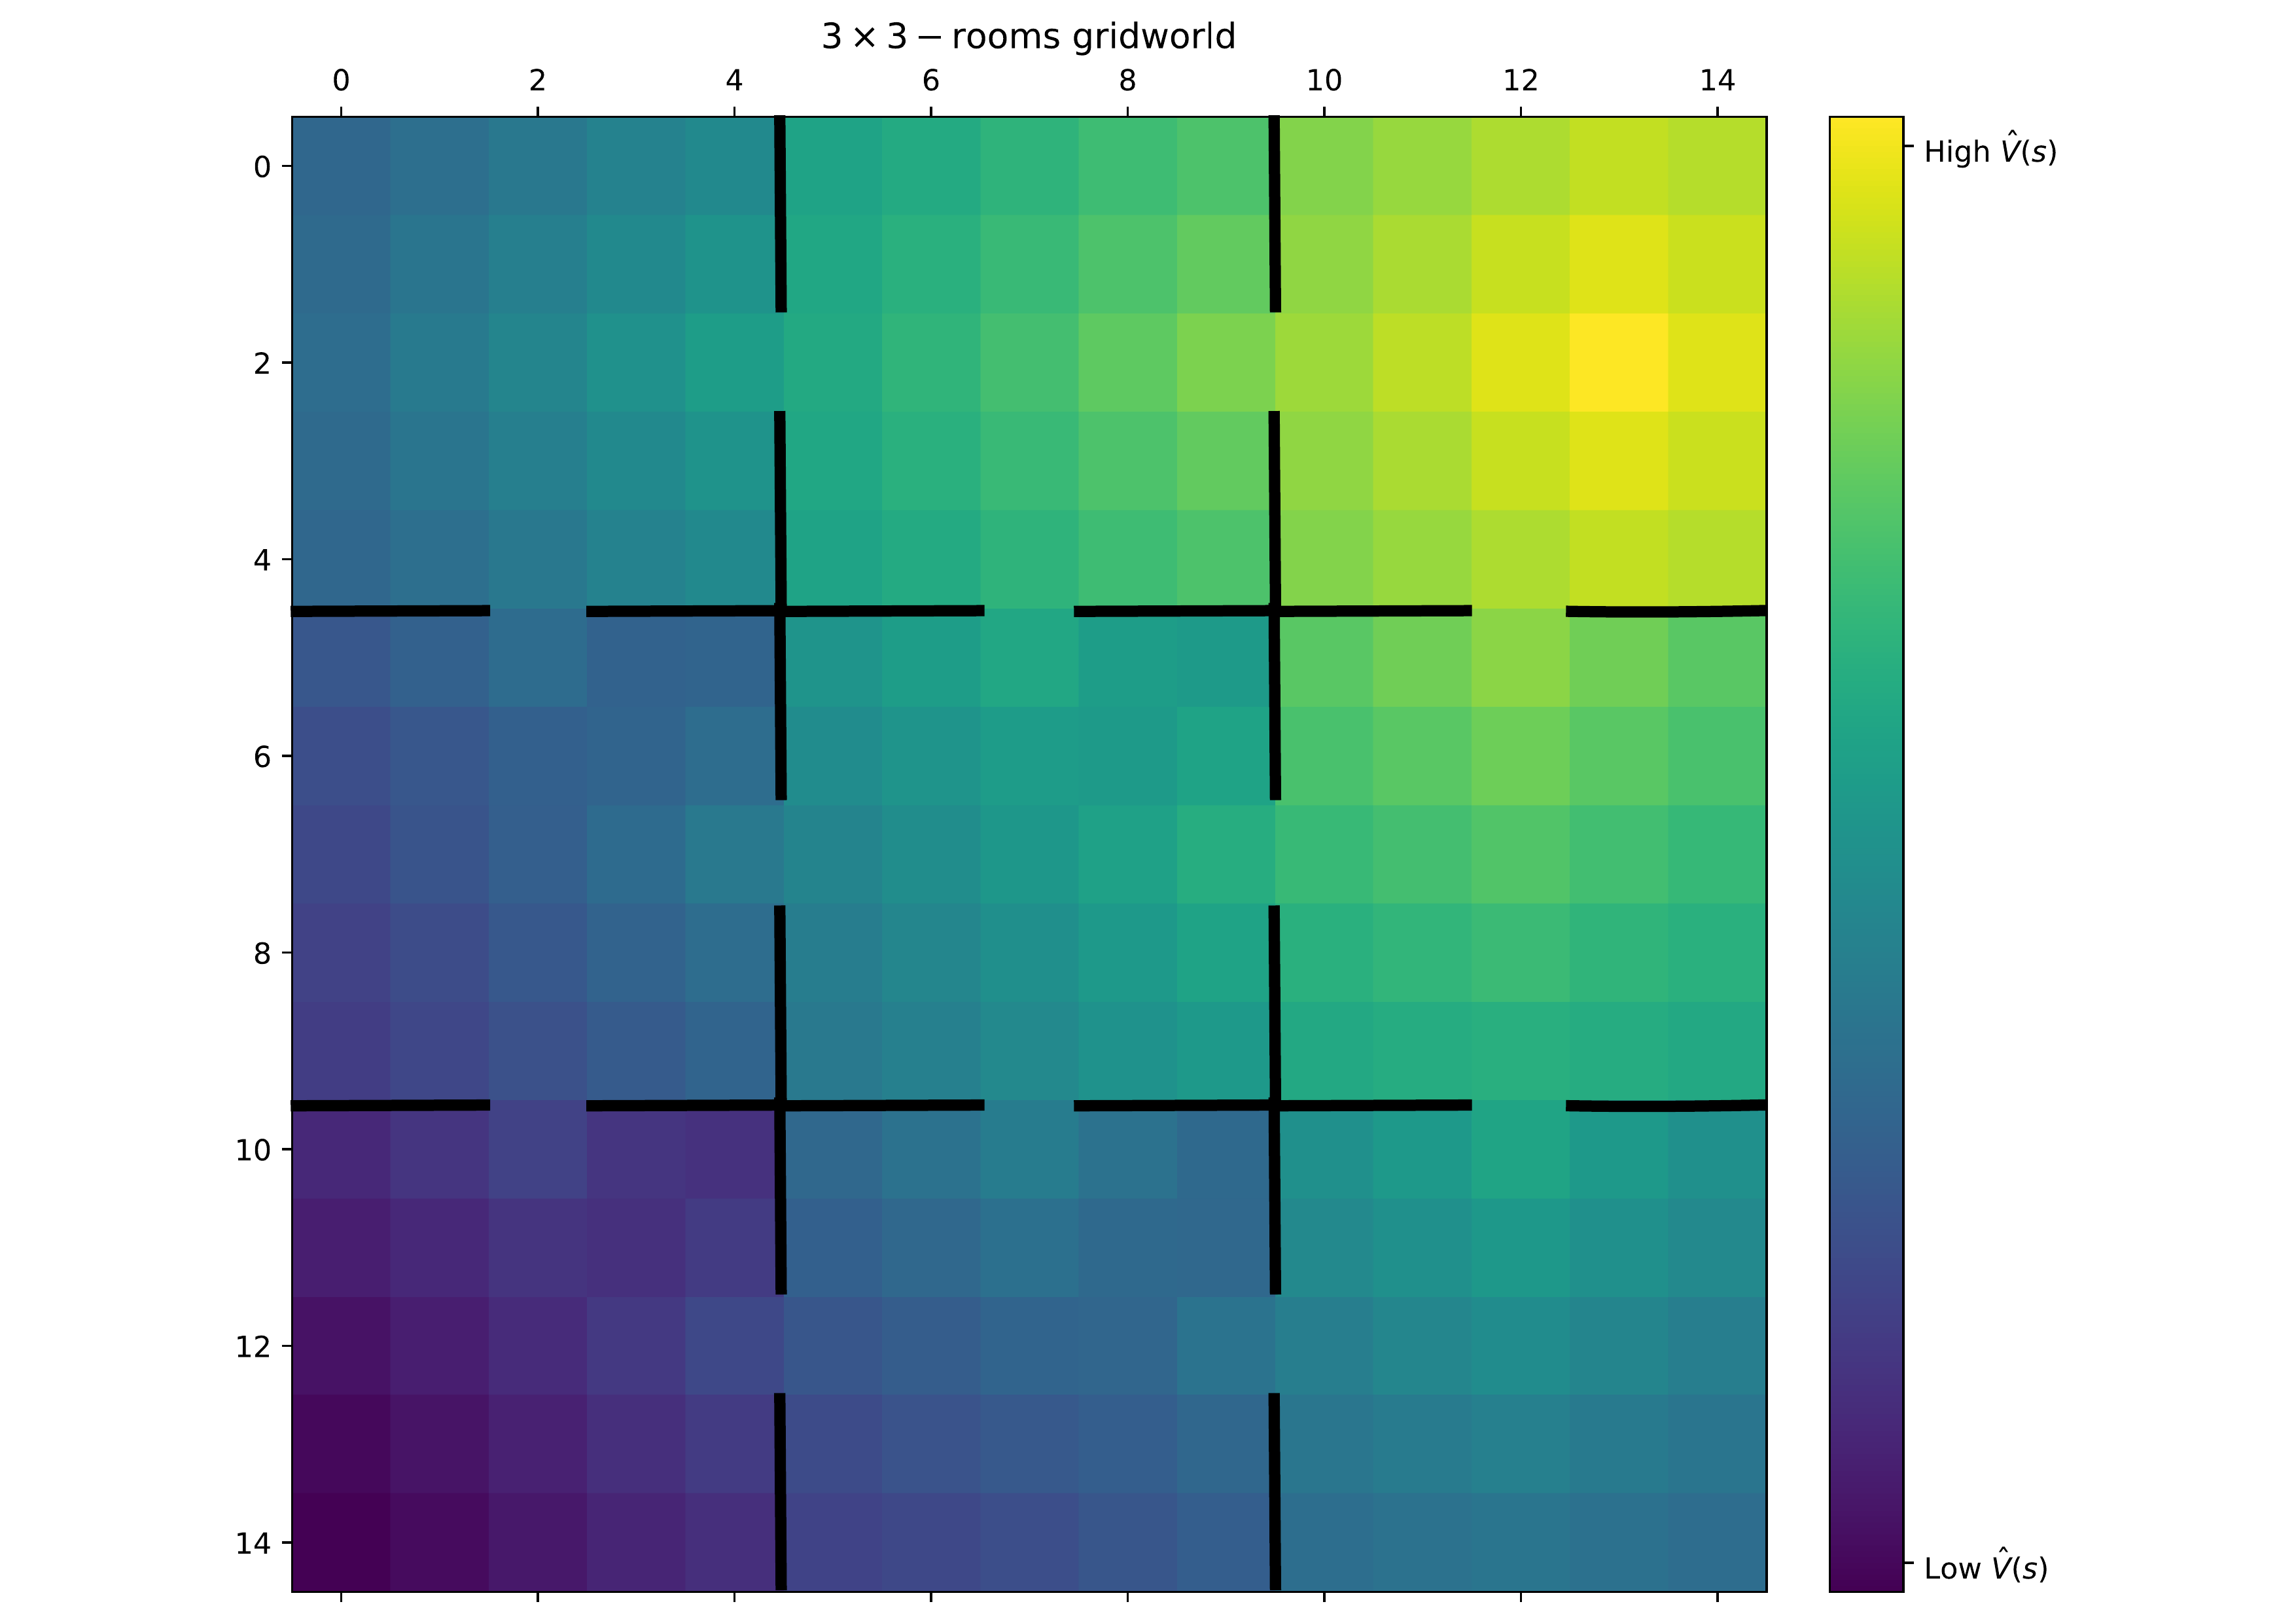
\includegraphics[scale=0.25]{Figures/grid_domain_VF.png}
%
%\label{fig:vf_grid}
%\end{figure}
%    
%\end{frame}

\begin{frame}{Results - Rooms domain}

    \begin{figure}[H]
        \centering
        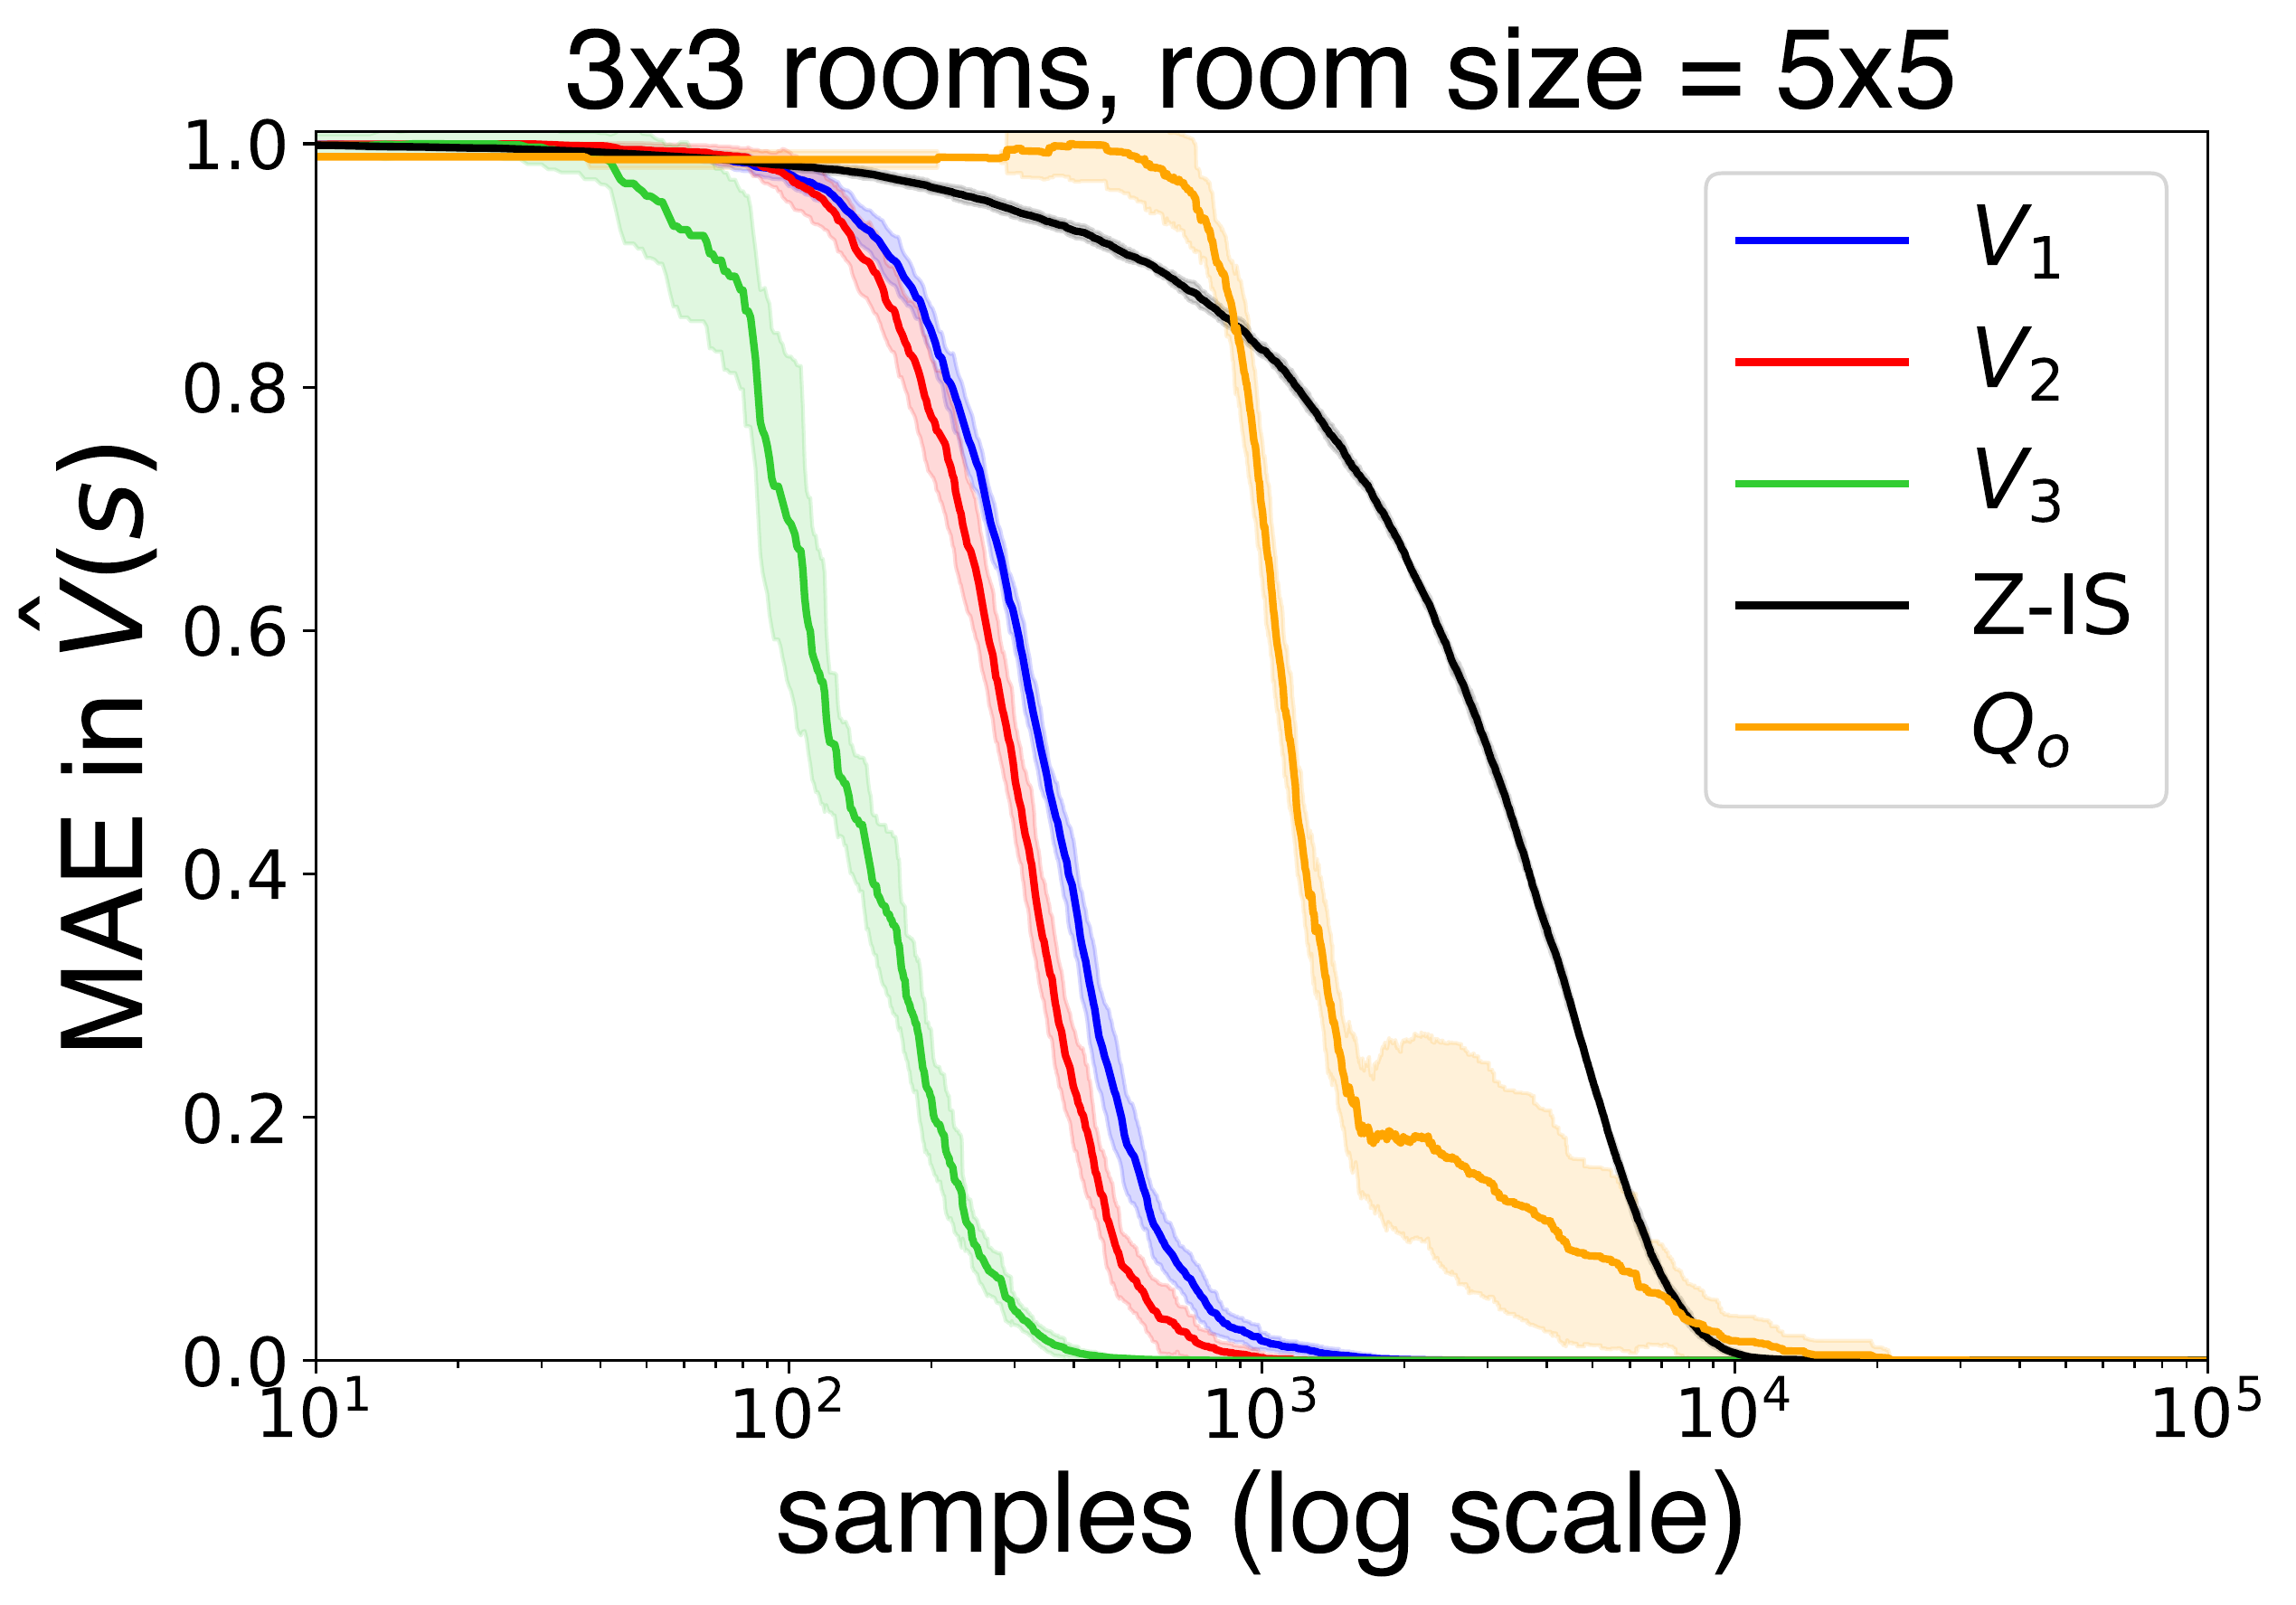
\includegraphics[scale=0.2]{Figures/nroom_3_3-1.png}
        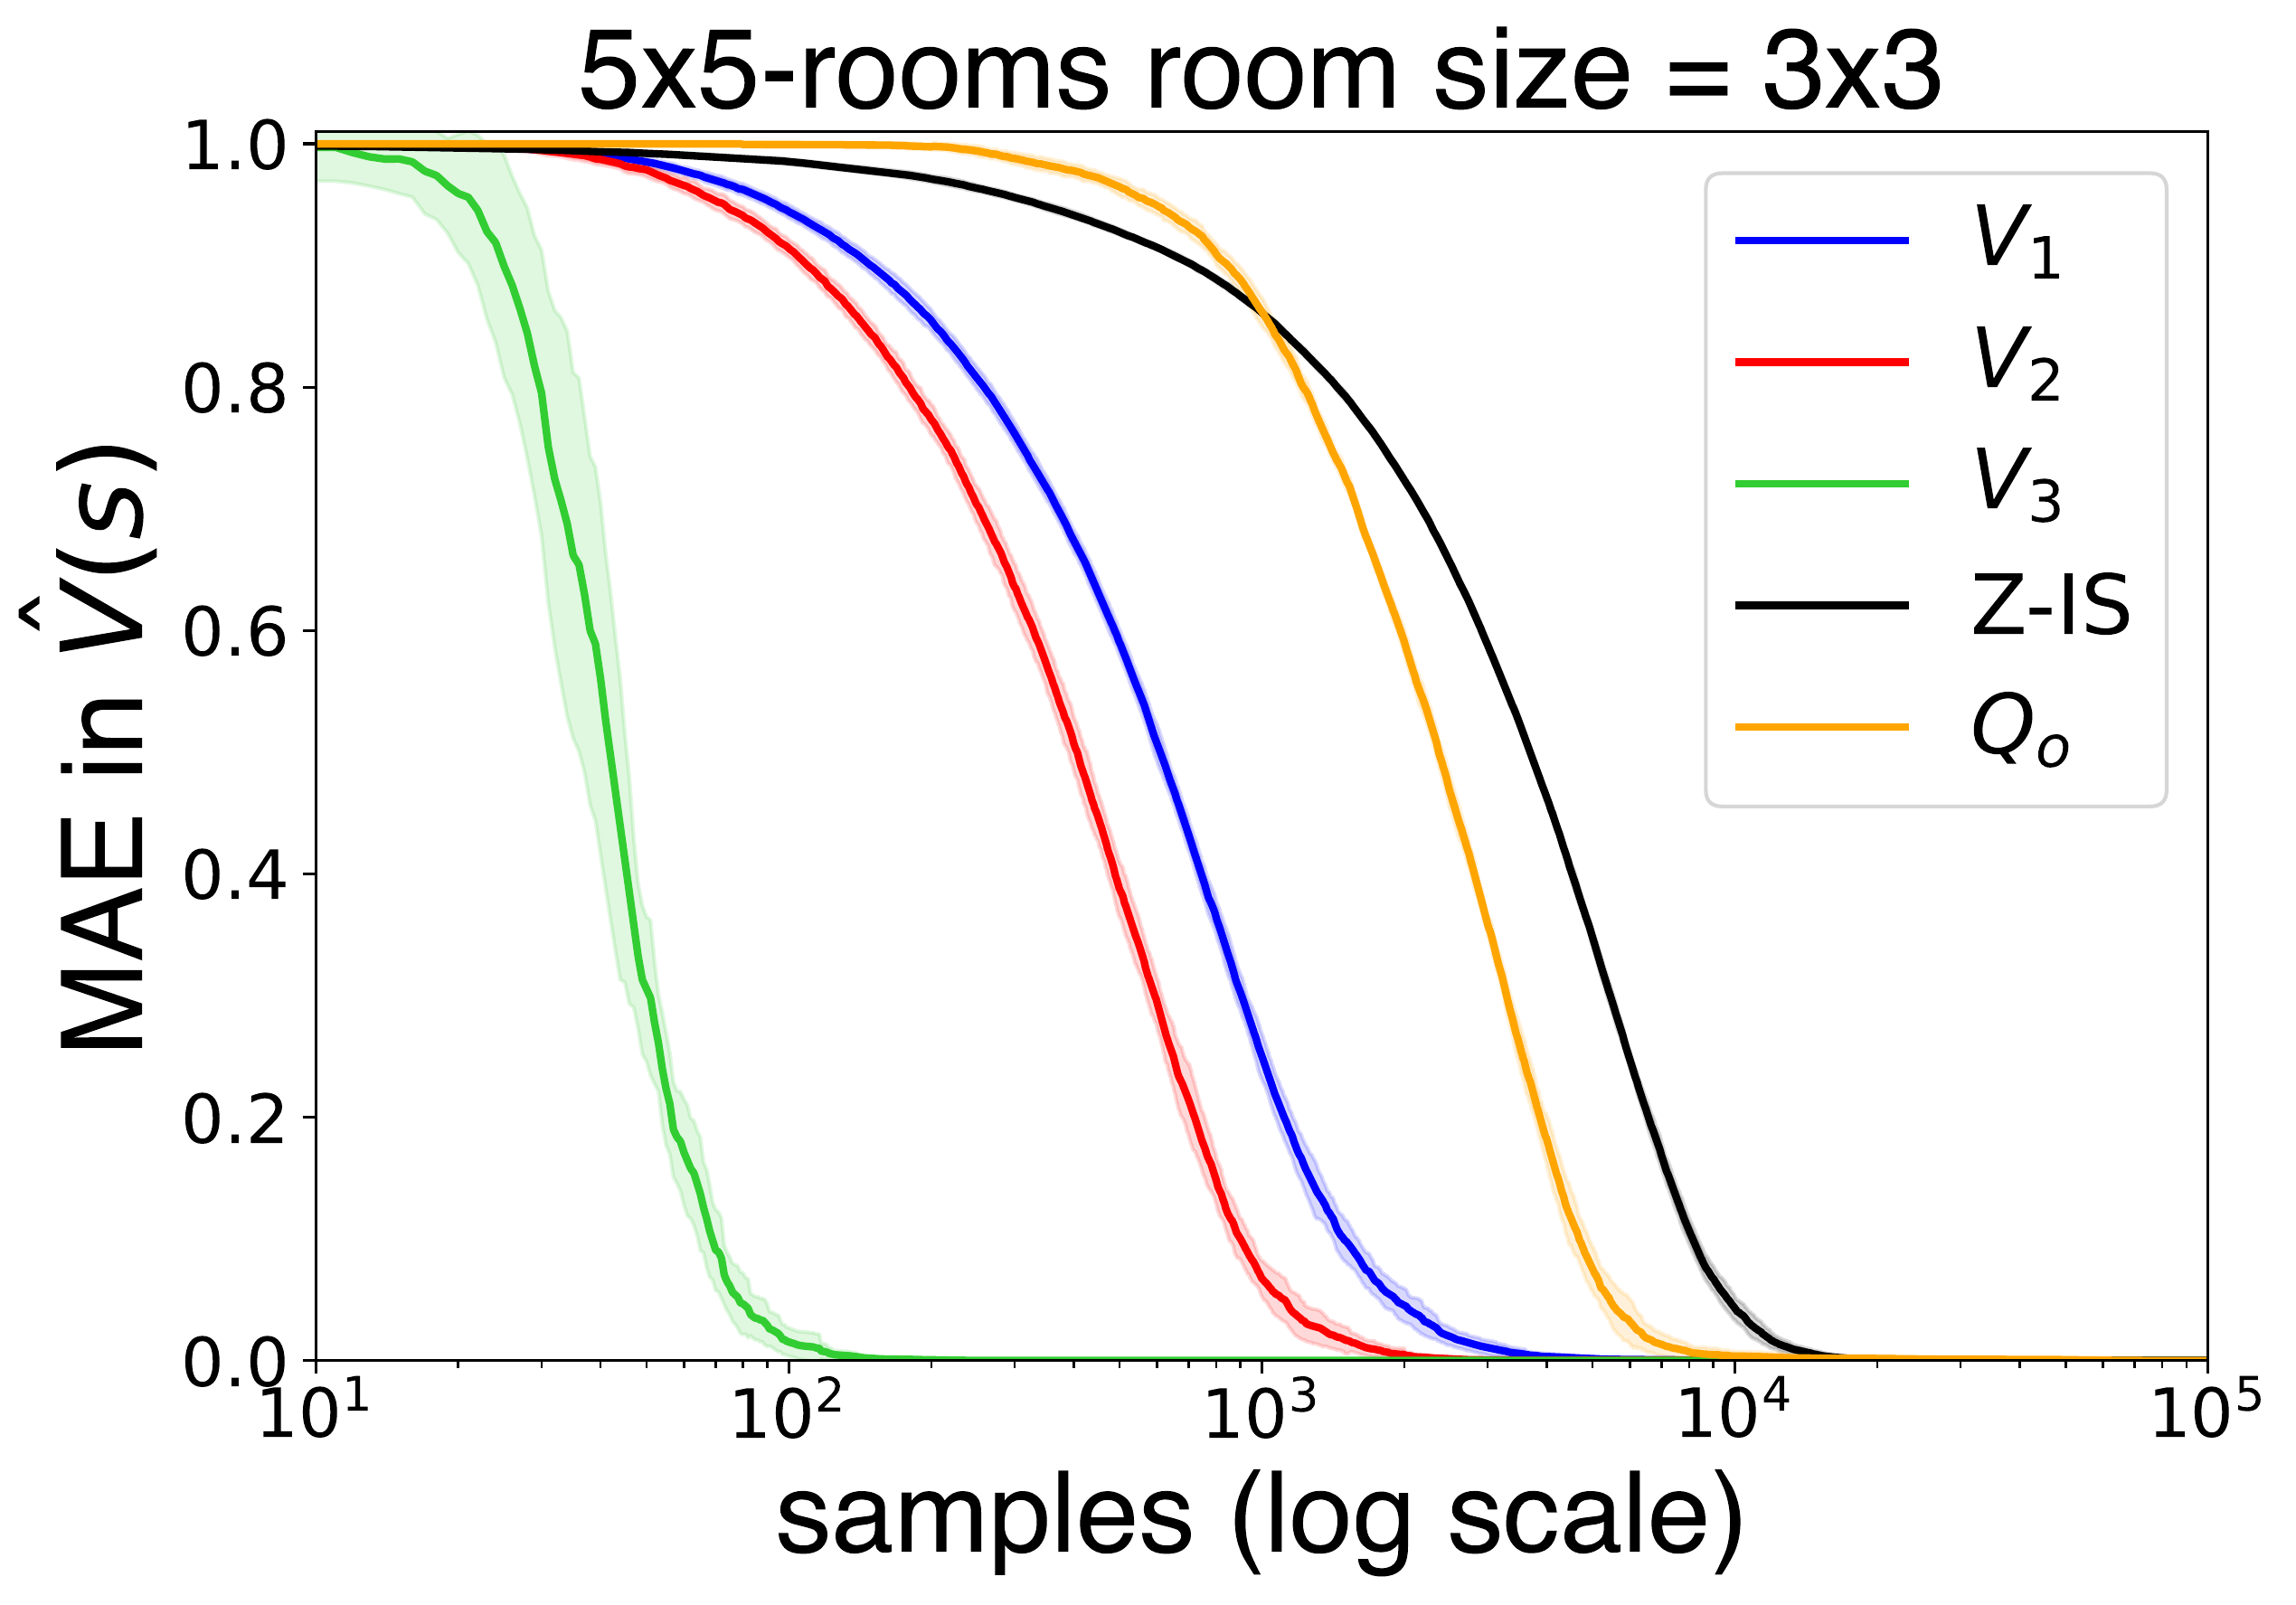
\includegraphics[scale=0.2]{Figures/nroom_5_5-1.png}
        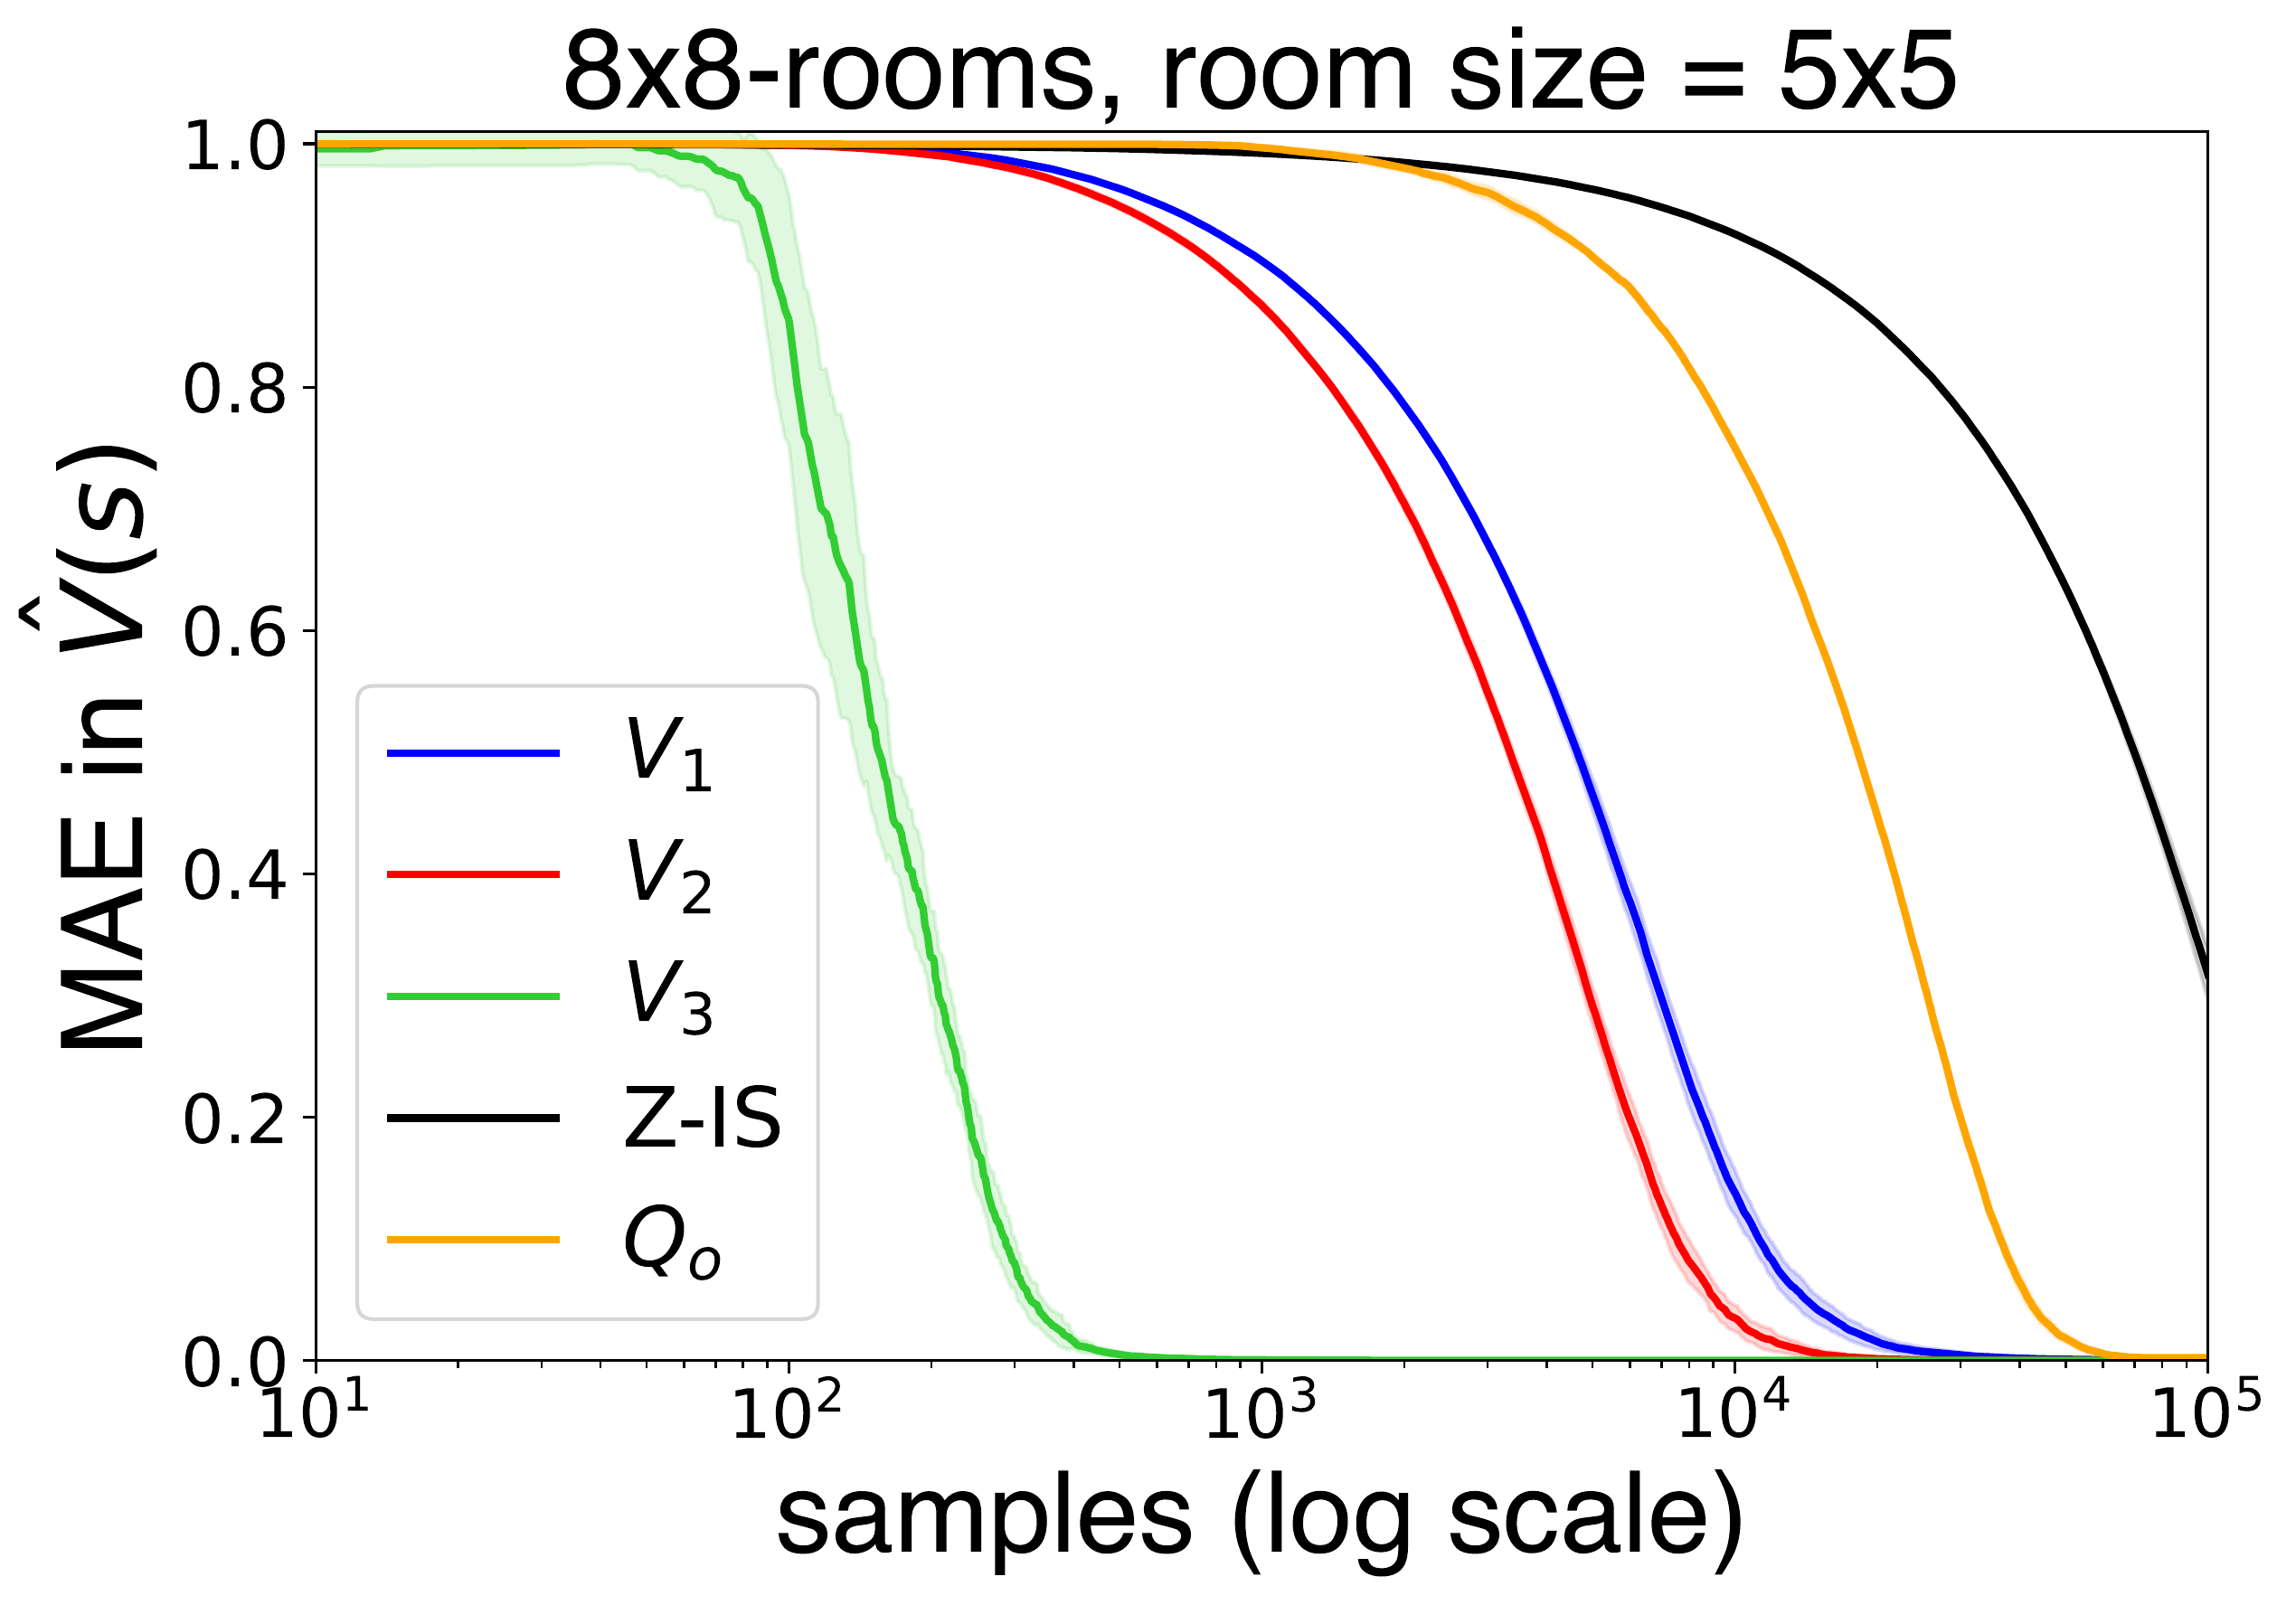
\includegraphics[scale=0.2]{Figures/nroom_8_8-1.png}

        \caption{MAE over time for $3 \times 3$ (top-left), $5 \times 5$ (top-right) and $8 \times 8$ (bottom) room instances.}
        \label{fig:errors_grid}
    \end{figure}

\end{frame}


\begin{frame}{Results - Taxi domain}

    \begin{figure}[H]
        \centering
        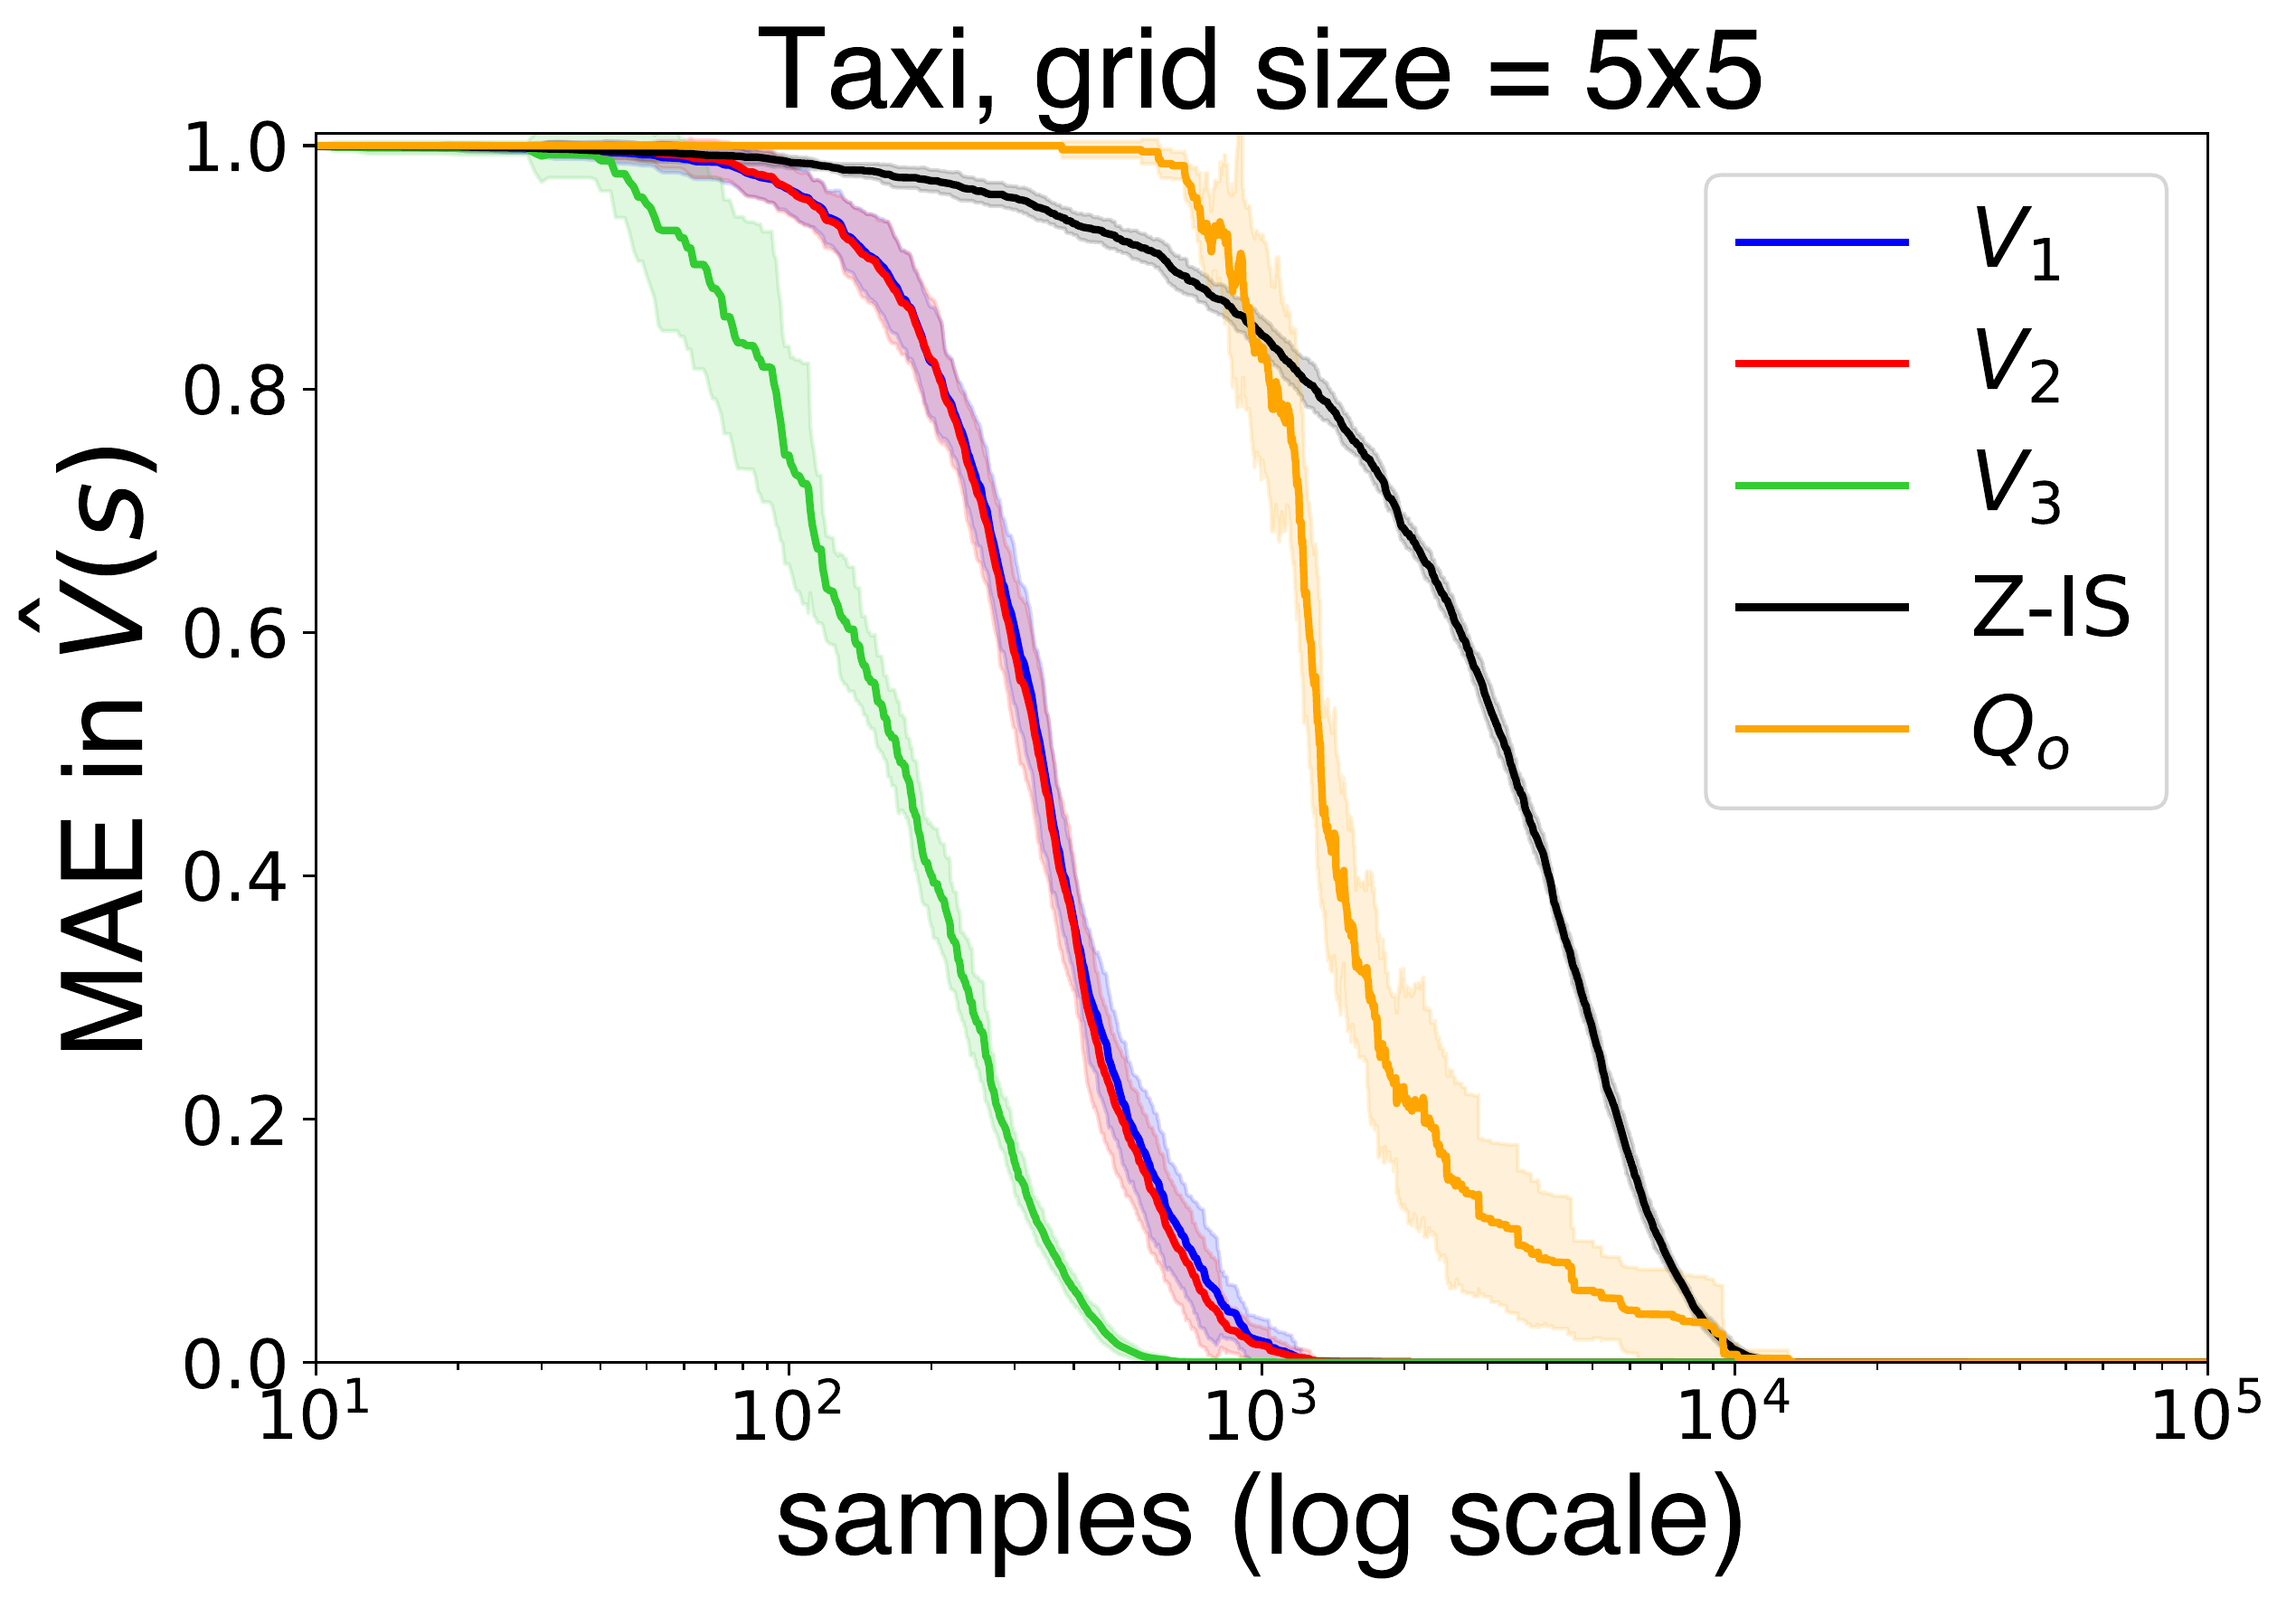
\includegraphics[scale=0.22]{Figures/taxi_5-1.png}
        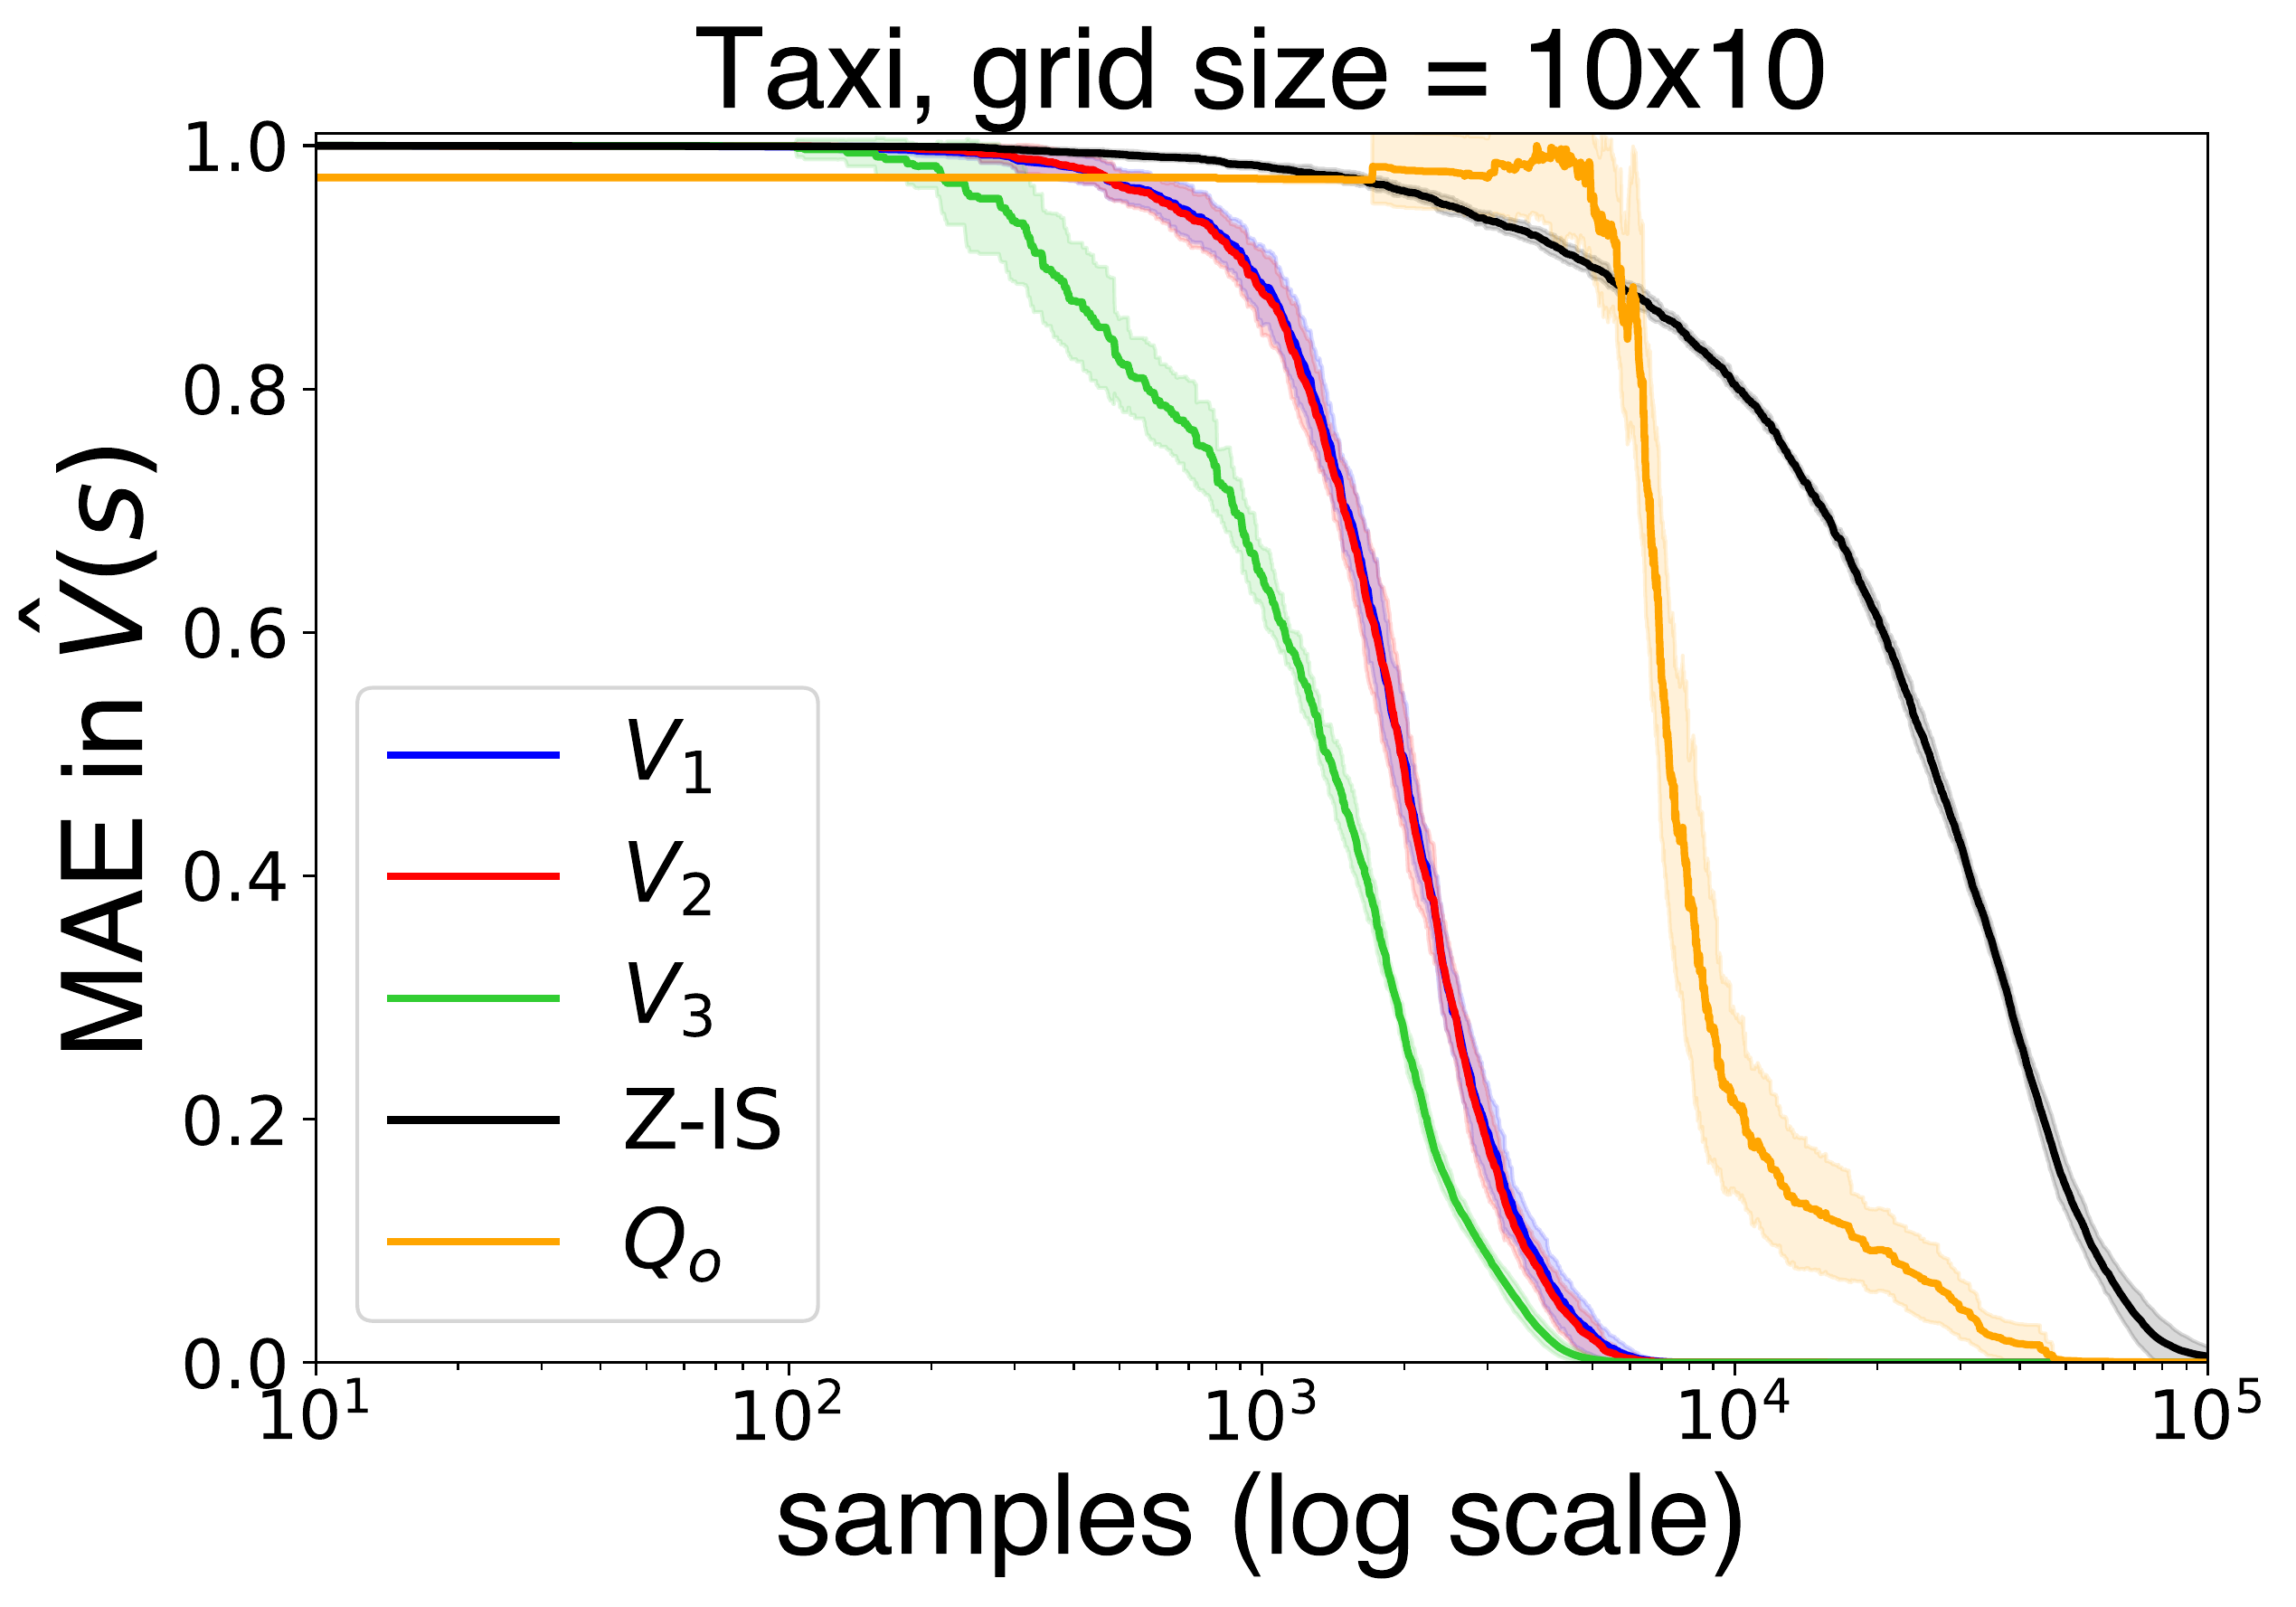
\includegraphics[scale=0.22]{Figures/taxi_10-1.png}
        \caption{MAE over time for $5 \times 5$ (left) and $10 \times 10$ (right) grids of Taxi domain.}
        \label{fig:errors_taxi}
    \end{figure}

\end{frame}

\section{Contributions and Conclusion}
\begin{frame}{Contributions}
    \begin{itemize}
        \item Novel scheme for hierarchical RL based on subtask compositionality.
        \item The subtasks decomposition is at the level of the value function.
        \item Our method converges to the optimal value function (vs.~recursively optimal solutions).
              %\item {\color{myred} Unlike the options setting, we can use the value estimates at exit states 
              %to retrieve $z$ for any $s \in \cS^+$.}
        \item More sample efficient algorithms.

    \end{itemize}

\end{frame}

\begin{frame}[allowframebreaks]{}
    \bibliographystyle{apalike}
    \bibliography{bibliography}
\end{frame}

\end{document}